Dado un sistema de transiciones $T$ que modela nuestro sistema, se quiere determinar si todas sus ejecuciones
 cumplen con una propiedad dada $\varphi$.
 
\[ ejecuciones(T) \subseteq \mathcal{L} (\varphi) \]

Este problema se puede ver como determinar si existe una ejecución del sistema que no cumple $\varphi$,
 o dicho de otra forma, que cumple $\lnot \varphi$.

\[ ejecuciones(T) \cap \mathcal{L} (\lnot \varphi) = \emptyset \]

El procedimiento para verificarlo consta de tres pasos. Cada uno de ellos se puede tratar
 de forma individual.

El primer paso es construir un NBA $\mathcal{A}$ que reconozca los malos comportamientos, esto es
 que reconozca las palabras que cumplen con $\lnot \varphi$. Este autómata es útil para encontrar las
 ejecuciones que no cumplen con la propiedad deseada.

A continuación se debe realizar el producto $T \otimes \mathcal{A}$, donde $T$ es el modelo de nuestro sistema
 y $\mathcal{A}$ el autómata obtenido en el paso anterior. De esta forma intersectamos las ejecuciones
 de nuestro sistema con las palabras que no cumplen la propiedad a verificar.

Por último debemos verificar que el lenguaje representado por el autómata resultante es vacío, esto significa
 que no hay ninguna ejecución del sistema que no cumple con la propiedad. En caso de no ser vacío, cualquiera
 de las palabras contenidas en él sirve como contraejemplo.
 %es una ejecución del sitema que no cumple con la propiedad.
 

\subsection{Construcción de un GNBA a partir de una fórmula LTL}

%- Conjuntos elementales
Veremos como construir un GNBA a partir de una fórmula $\varphi$.

Lo primero es calcular el conjunto $clausura( \varphi )$ que se define a continuación.

\begin{definicion}
Clausura. \\
La clausura de una fórmula LTL es el conjunto formado por todas sus subfórmulas y sus negaciones.
\end{definicion}

Ahora se necesita construir los conjuntos elementales con respecto a $clausura( \varphi )$.\\

\begin{definicion}
Conjunto elemental.\\
Sea $B$ un subconjunto de la clausura $\varphi$.
$B$ es un conjunto elemental de $\varphi$ si cumple:
\begin{itemize}
\item es consistente con respecto a la lógica proposicional:
	\begin{itemize}
	\item $\varphi_1 \wedge \varphi_2 \in B \Longleftrightarrow \varphi_1 \in B$ y $\varphi_2 \in B$
	\item $\neg \psi \in B \Longrightarrow \psi \not\in B$
	\item $true \in clausura(\varphi ) \Longrightarrow true \in B$
	\end{itemize}
\item es maximal:
	\begin{itemize}
	\item $\varphi_2 \in B \Longrightarrow \varphi_1 \cup \varphi_2 \in B$
	\item $\varphi_1 \cup \varphi_2 \in B$ y $\varphi_2 \not\in B \Longrightarrow \varphi_1 \in B$
	\end{itemize}
\item es localmente consistente con respecto al operador until:
	\begin{itemize}
	\item $\psi \not\in B \Longrightarrow \neg \psi \in B$
	\end{itemize}
\end{itemize}
\end{definicion}



%- Reglas para construirlos
%figura 5.20


% construccion del gnba - página 278
Una vez definidos los conceptos anteriores se puede comenzar a construir el GNBA para una
fórmula LTL de la siguiente manera:
\begin{enumerate}
\item El conjunto de estado está formado por todos los conjuntos de fórmulas elementales de
 $\varphi$
\item $Q_0 = \{ B \in Q | \varphi \in B \}$ \\
El conjunto de estados iniciales está formado por todos los estados que contienen a $\varphi$
\item $F = \{ F_{\varphi_1 \cup \varphi_2} | \varphi_1 \cup \varphi_2 \in clausura(\varphi) \}$ donde 
$F_{\varphi_1 \cup \varphi_2} = \{ B \in Q | \varphi_1 \cup \varphi_2 \not\in B$ o $ \varphi_2 \in B\}$ \\
es el conjunto de aceptación
\item La relación de trasición $\delta : Q \times 2^{AP} \rightarrow 2^Q$ queda definida por:
\begin{itemize}
\item si $A \neq B \cap AP$ entonces $\delta (B,A) = \phi$
\item si $A = B \cap AP$ entonces $\delta (B,A) = B'$, donde $B'$ es el conjunto elemental de fórmulas
que cumple:
\begin{itemize}
\item[i] para cada $\bigcirc \psi \in clausura(\varphi) : \bigcirc \psi \in B \Leftrightarrow \psi \in B'$ y
\item[ii] para cada $\varphi_1 \cup \varphi_2 \in clausura(\varphi ):$ \\
$\varphi_1 \cup \varphi_2 \in B \Leftrightarrow (\varphi_2 \in B \vee (\varphi_1 \in B \wedge \varphi_1 \cup \varphi_2 \in B'))$
\end{itemize}
\end{itemize}
\end{enumerate}

Con este mecanismo podemos generar un GNBA para cualquier fórmula LTL, asumiendo que estas fórmulas LTL
 contienen únicamente los conectivos $true$, $\lnot$, $\land$, $\bigcirc$ y $\cup$. En caso de que esto
 no se cumpla, se puede generar un GNBA para una fórmula equivalente que utilice sólo estos conectivos
 con las propiedades vistas anteriormente.

\paragraph{Ejemplo.}
Considerando la fórmula $\varphi = a \cup b$.\\
Los conjuntos de fórmulas elementales de $\varphi$ son:
\[
B_1 = \{ a, b, \varphi \}, 
B_2 = \{ \lnot a, b, \varphi \}, 
B_3 = \{ a, \lnot b, \varphi \}, 
B_4 = \{ \lnot a, \lnot b, \lnot \varphi \}, 
B_5 = \{ a, \lnot b, \lnot \varphi \}
\]

Los estados iniciales son los conjuntos $B_i$ tal que $\varphi \in B_i$. $Q_0 = \{ B_1, B_2, B_3 \}$.

El conjunto de conjuntos de aceptación es $F = \{ F_\varphi \}$, donde
\[ F_\varphi = \{ B \in Q | \varphi \in B \vee q \in B \} = \{ B_1, B_2, B_4, B_5 \} \]
El GNBA resultante se muestra en la figura \ref{fig:GNBA_formula}.
\begin{figure}[hbtp]
\begin{minipage}{\textwidth}
\begin{center}
\caption[GNBA para la fórmula $ a \cup b $]%
{GNBA para la fórmula $ a \cup b $ \footnote[1]{Imagen tomada de \cite{katoen}}}
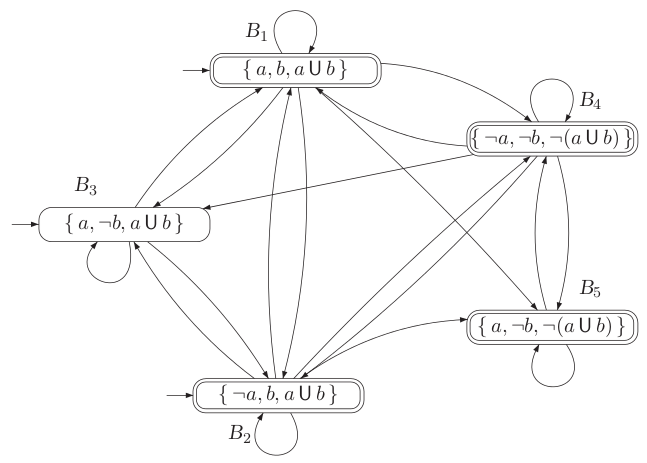
\includegraphics[width=0.8\textwidth]{ltl/imagenes/figura5_22.png}
\label{fig:GNBA_formula}
\end{center}
\end{minipage}
\end{figure}


%Luego se debe determinar si las trazas del sistema de transiciones T no contienen ninguna palabra
% que sea reconocida por A, o sea un mal comportamiento de nuestro sistema.

Una vez obtenido el GNBA para una fórmula $\varphi$ debemos transformar este en un NBA equivalente.
Para esto primero debemos entender la principal dieferencia entre ambos.
Esta radica en su criterio de aceptación. Una palabra es reconocida (o aceptada) por un NBA si esta
pasa infinitas veces por al menos un estado de su conjunto de aceptación. Mientras que una palabra
es reconocida por un GNBA si esta pasa infinitas veces por al menos un estado de cada conjunto de
 aceptación.

Sabiendo esto se puede encontrar un método sencillo para transformar un GNBA en un NBA equivalente.

Sea $\mathcal(G)$ un GNBA y $\mathcal(F) = \{ F_1 , ..., F_k \} $ el conjunto formado por todos sus
 estados de aceptación.
El método consiste en crear $k$ copias de $\mathcal(G)$ tales que cada estado del conjunto $F_i$ está
 conectado con los correspondientes estados en la copia $i + 1$ como se muestra en la
 figura \ref{fig:GNBA_to_NBA}.

%IMAGEN pag 195
\begin{figure}[hbtp]
\begin{minipage}{\textwidth}
\begin{center}
\caption[Generación de un NBA a partir de un GNBA]%
{Generación de un NBA a partir de un GNBA \footnote[1]{Imagen tomada de \cite{katoen}}}
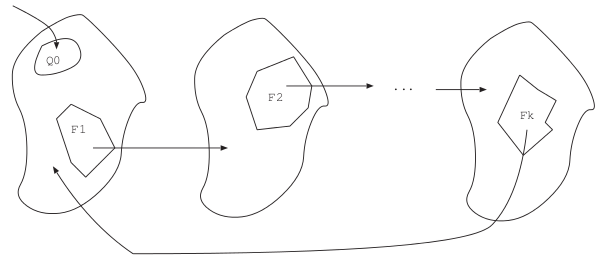
\includegraphics[width=0.8\textwidth]{ltl/imagenes/figura4_20.png}
\label{fig:GNBA_to_NBA}
\end{center}
\end{minipage}
\end{figure}

El conjunto de aceptación del NBA resultante es el conjunto $F_1$ de la copia 1.

De esta forma nos aseguramos de que toda palabra que pase infinitas veces por alguno de los estados
 de $F_1$ pasa infitas veces por al menos un estado de cada conjunto de aceptación de $\mathcal{G}$.



\subsection{Producto}

En segundo lugar se realiza el producto $T \otimes \mathcal{A}$, siendo $\mathcal{A}$ el NBA resultante
 de la parte anterior.

El lenguaje reconocido por el producto de dos autómatas es la intersección de los lenguajes reconocidos
 por cada uno de ellos.

El producto $\mathcal{A} = \mathcal{A}_1 \otimes \mathcal{A}_2 $ queda definido de la siguiente manera
\begin{itemize}
\item El conjunto de estados $Q = Q_1 \times Q_2$ siendo $Q_1$ y $Q_2$ los conjuntos de estados de
 $\mathcal{A}_1$ y $\mathcal{A}_2$ respectivamente.
\item El conjunto de estados iniciles $Q_0 = Q_{0_1} \times Q_{0_2}$ siendo $Q_{0_1}$ y $Q_{0_2}$ los conjuntos
 de estados iniciales de $\mathcal{A}_1$ y $\mathcal{A}_2$ respectivamente.
\item La función de transición $\delta$ cumple
\[  \delta_1(q_1, A) = q'_1 ~~  y ~~ \delta_2(q_2, A) = q'_2 ~~ entonces ~~ \delta((q_1,q_2), A) = (q'_1,q'_2)\]
\item En este proyecto se trabaja con sistemas reactivos, y al estos no tener estados finales, el conjunto de
 aceptación es $F= \{ (q_1,q_2) | q_1 \in F_1 \}$ siendo $F_1$ el conjunto de aceptción de $\mathcal{A}_1$.
\end{itemize}


\subsection{Algoritmo de verificación}
Por último se debe verificar si las trazas del sistema de transiciones $T$ no contienen ninguna palabra
 que sea reconocida por $\mathcal{A}$, o sea un mal comportamiento de nuestro sistema. Esto significa que
 ninguna ejecución de $T$ es reconocida por el autómata $\mathcal{A}$.

Lo anterior es equivalente a controlar que $T \otimes \mathcal{A} \models \lozenge \box \lnot F$
 siendo $F$ un estado de aceptación.
Esto se logra verificando si existe algún estado de aceptación alcanzable y que al mismo tiempo pertenezca
 a un ciclo.
 
